\documentclass[11pt]{article}
\usepackage[margin=0.9in]{geometry}
\usepackage[T1]{fontenc}
\usepackage{lmodern,microtype,amsmath,amssymb,booktabs,graphicx,array,float}
\usepackage[colorlinks=true,linkcolor=blue,citecolor=blue,urlcolor=blue]{hyperref}
\hypersetup{pdftitle={Heat-Kernel Cryptanalysis of SHA-256: A Geometric Study of State Evolution},pdfauthor={Bee Rosa Davis},pdfkeywords={SHA-256, heat-kernel cryptanalysis, spectral geometry, state evolution, avalanche effect, higher-order differentials}}
\usepackage[font=small,labelfont=bf]{caption}
\usepackage[section]{placeins}
\setlength{\parskip}{4pt}
\setlength{\parindent}{0pt}
\setlength{\emergencystretch}{2em}
\setcounter{topnumber}{4}
\setcounter{totalnumber}{5}
\renewcommand{\topfraction}{0.9}
\renewcommand{\textfraction}{0.07}
\renewcommand{\floatpagefraction}{0.8}
\newcommand{\HoldoutDifference}{+0.009}
\newcommand{\HoldoutCI}{[-0.2869, 0.3140]}
\newcommand{\SearchDifference}{+0.126}
\newcommand{\SearchCI}{[-0.4354, 0.6657]}
\newcommand{\FinalHamming}{128.024}
\newcommand{\RFAccuracy}{50.315}
\newcommand{\SVMAccuracy}{49.800}
\newcommand{\GraphRows}{%
Primary & 1.0 & Silhouette & 0.8957 & 0.9066 & -0.0110 [-0.0439, 0.0196] \\
Primary & 1.0 & Gap & 0.2050 & 0.2046 & +0.0003 [-0.0349, 0.0422] \\
Primary & 8.0 & Silhouette & 0.1608 & 0.1635 & -0.0028 [-0.0047, -0.0010] \\
Primary & 8.0 & Gap & 0.6159 & 0.6139 & +0.0020 [-0.0009, 0.0051] \\
Primary & -- & Detour & 2.5629 & 2.5660 & -0.0031 [-0.0053, -0.0008] \\
Confirmation & 1.0 & Silhouette & 0.8803 & 0.8985 & -0.0182 [-0.0471, 0.0059] \\
Confirmation & 1.0 & Gap & 0.2461 & 0.2246 & +0.0215 [-0.0145, 0.0599] \\
Confirmation & 8.0 & Silhouette & 0.1654 & 0.1647 & +0.0007 [-0.0030, 0.0049] \\
Confirmation & 8.0 & Gap & 0.6145 & 0.6153 & -0.0008 [-0.0032, 0.0017] \\
Confirmation & -- & Detour & 2.5640 & 2.5674 & -0.0034 [-0.0065, -0.0006] \\%
}
\newcommand{\SensitivityRows}{%
state -- PCG64 & -0.00045 & [-0.0032, 0.0025] \\
state -- MT19937 & +0.00042 & [-0.0026, 0.0033] \\
digest -- PCG64 & +0.00092 & [-0.0027, 0.0045] \\
digest -- MT19937 & +0.00179 & [-0.0010, 0.0044] \\
PCG64 -- MT19937 & +0.00087 & [-0.0019, 0.0036] \\%
}
\newcommand{\CubeRows}{%
8 & 48.83 & 49.52 & -0.69 & [-5.21, 3.68] & 1.000 \\
10 & 46.48 & 50.58 & -4.09 & [-8.74, 0.36] & 0.975 \\
12 & 53.12 & 49.07 & +4.05 & [-0.41, 8.36] & 1.000 \\
14 & 47.07 & 49.20 & -2.13 & [-6.48, 2.30] & 1.000 \\
16 & 51.56 & 50.06 & +1.50 & [-3.10, 5.97] & 1.000 \\
18 & 49.80 & 49.59 & +0.21 & [-4.19, 4.46] & 1.000 \\
20 & 47.46 & 50.52 & -3.06 & [-7.38, 1.41] & 1.000 \\
24 & 52.54 & 49.94 & +2.60 & [-1.75, 7.01] & 1.000 \\%
}
\newcommand{\MLRows}{%
RF & 50.315 & 49.825--51.050 & 0.5017 \\
PCA + SVM & 49.800 & 48.225--51.425 & 0.5003 \\%
}

\newcommand{\PositionSD}{0.697}
\newcommand{\NoiseFloor}{0.706}
\newcommand{\RoundCorrelation}{0.018}
\newcommand{\FreshDetourMean}{-0.00032}
\newcommand{\FreshDetourCI}{[-0.00168, +0.00098]}
\newcommand{\EarlyCubeTarget}{90.43}
\newcommand{\EarlyCubeControl}{72.29}
\newcommand{\EarlyCubeDifference}{18.14}
\newcommand{\EarlyCubeCI}{[+15.449, +20.752]}
\newcommand{\EarlyCubeP}{$2.03\times10^{-84}$}
\newcommand{\MatchedSearchDiffTwo}{+1.55}
\newcommand{\MatchedSearchCITwo}{[+1.14, +1.96]}
\newcommand{\MatchedSearchBelowTwo}{36}
\newcommand{\UniformSearchOffsetCorr}{0.50}
\newcommand{\UniformCubeMinTwo}{50.98}
\newcommand{\UniformCubeMaxTwo}{96.09}
\newcommand{\UniformCubeAboveCorr}{0.40}
\newcommand{\MatchedCubeMeanTwo}{86.08}
\newcommand{\MatchedCubeRangeTwo}{49.6--94.9}
\newcommand{\MatchedCubeAtOrAboveTwo}{19}
\newcommand{\MatchedCubeDiffTwo}{+4.35}
\newcommand{\MatchedCubeCITwo}{[+1.8, +6.8]}
\newcommand{\WholeWordATwo}{0.20}
\newcommand{\WholeWordAControlTwo}{0.27}
\newcommand{\MatchedCubeRankCITwo}{13--26}
\newcommand{\MatchedSearchRankCITwo}{33--38}
\newcommand{\MatchedCubeSevenDiff}{+4.86}
\newcommand{\MatchedCubeSevenCI}{[+0.4, +9.3]}
\newcommand{\EarlyCorrRange}{0.930--0.979}
\newcommand{\EarlyCorrSix}{0.557}
\newcommand{\EarlyCorrSeven}{-0.017}
\newcommand{\PrimaryOneSizesSHA}{(2.00,2.05,2.30,3.65,502.00)}
\newcommand{\ConfirmationLargestSHA}{500.95}
\newcommand{\PrimaryEightRangeSHA}{86.40 to 121.20}
\newcommand{\PrimaryOneSizesRandom}{(2.00,2.05,2.10,3.55,502.30)}
\newcommand{\ConfirmationLargestRandom}{501.85}
\newcommand{\PrimaryEightRangeRandom}{81.35 to 121.05}
\newcommand{\HeatTraceRows}{%
Primary & 1 & 0.01 & $10^{-5}$ & -1.798 & [-8.787, +5.430] \\
Primary & 1 & 0.1 & $10^{-3}$ & -1.645 & [-8.039, +4.968] \\
Primary & 1 & 1 & $10^{-1}$ & -0.707 & [-3.428, +2.104] \\
Primary & 1 & 10 & $10^{-1}$ & -0.199 & [-1.697, +1.406] \\
Primary & 8 & 0.01 & $10^{-7}$ & -2.993 & [-8.974, +3.355] \\
Primary & 8 & 0.1 & $10^{-5}$ & -2.776 & [-8.243, +3.022] \\
Primary & 8 & 1 & $10^{-3}$ & -1.319 & [-3.600, +1.039] \\
Primary & 8 & 10 & $10^{-4}$ & -1.051 & [-3.177, +1.121] \\
Confirmation & 1 & 0.01 & $10^{-5}$ & -1.212 & [-7.183, +4.511] \\
Confirmation & 1 & 0.1 & $10^{-3}$ & -1.114 & [-6.569, +4.111] \\
Confirmation & 1 & 1 & $10^{-1}$ & -0.520 & [-2.810, +1.664] \\
Confirmation & 1 & 10 & $10^{-1}$ & -0.643 & [-1.527, +0.246] \\
Confirmation & 8 & 0.01 & $10^{-6}$ & -0.617 & [-1.395, +0.103] \\
Confirmation & 8 & 0.1 & $10^{-4}$ & -0.564 & [-1.278, +0.100] \\
Confirmation & 8 & 1 & $10^{-3}$ & -2.316 & [-5.353, +0.582] \\
Confirmation & 8 & 10 & $10^{-4}$ & -1.128 & [-3.546, +1.472] \\%
}
\newcommand{\EarlyCoordinateRows}{%
1 & 0.973 & 2.00 & 3.77 & 0 & 0 \\
2 & 0.979 & 19.00 & 24.89 & 0 & 0 \\
3 & 0.962 & 48.45 & 55.57 & 0 & 0 \\
4 & 0.964 & 80.34 & 87.40 & 0 & 0 \\
5 & 0.930 & 110.20 & 115.62 & 0 & 0 \\
6 & 0.557 & 125.05 & 126.51 & 13 & 0 \\
7 & -0.017 & 127.12 & 127.88 & 22 & 15 \\%
}
\newcommand{\EarlySearchRows}{%
2 & 23.66 & 24.87 & -1.22 [-1.65, -0.79] & 22.11 & +1.55 [+1.14, +1.96] & 36/40 \\
3 & 51.85 & 53.57 & -1.72 [-2.30, -1.16] & 50.54 & +1.31 [+0.78, +1.85] & 34/40 \\
4 & 81.96 & 83.81 & -1.85 [-2.53, -1.18] & 80.85 & +1.11 [+0.47, +1.74] & 31/40 \\
5 & 107.15 & 108.43 & -1.28 [-1.92, -0.64] & 106.69 & +0.46 [-0.19, +1.09] & 28/40 \\
6 & 113.36 & 113.74 & -0.38 [-0.92, +0.17] & 113.55 & -0.20 [-0.68, +0.32] & 13/40 \\
7 & 113.97 & 114.07 & -0.10 [-0.65, +0.44] & 114.02 & -0.05 [-0.56, +0.45] & 18/40 \\
24 & 114.52 & 114.20 & +0.32 [-0.19, +0.81] & 114.18 & +0.34 [-0.16, +0.83] & 38/40 \\%
}
\newcommand{\EarlyCubeRows}{%
2 & 90.43 & 72.29 & +18.14 [+15.4, +20.8] & 86.08 & +4.35 [+1.8, +6.8] & 19/40 & $2.03\times10^{-84}$ \\
3 & 50.00 & 49.23 & +0.77 [-3.8, +5.0] & 50.37 & -0.37 [-4.8, +3.9] & 24/40 & 1.000 \\
4 & 52.15 & 49.74 & +2.41 [-2.2, +6.8] & 49.64 & +2.51 [-2.1, +6.8] & 6/40 & 1.000 \\
5 & 52.34 & 49.84 & +2.50 [-1.9, +6.9] & 49.36 & +2.99 [-1.4, +7.4] & 3/40 & 1.000 \\
6 & 53.71 & 49.34 & +4.38 [-0.2, +8.6] & 49.88 & +3.83 [-0.7, +8.1] & 3/40 & 1.000 \\
7 & 54.30 & 50.92 & +3.38 [-1.3, +7.9] & 49.44 & +4.86 [+0.4, +9.3] & 0/40 & 0.745 \\
8 & 48.83 & 49.43 & -0.61 [-5.2, +3.9] & 49.99 & -1.16 [-5.6, +3.3] & 30/40 & 1.000 \\
10 & 50.78 & 50.16 & +0.62 [-3.8, +5.1] & 49.98 & +0.81 [-3.6, +5.2] & 15/40 & 1.000 \\
12 & 50.78 & 49.57 & +1.21 [-3.3, +5.7] & 50.29 & +0.49 [-3.9, +5.0] & 17/40 & 1.000 \\
14 & 53.12 & 50.21 & +2.91 [-1.6, +7.2] & 49.75 & +3.38 [-1.2, +7.7] & 4/40 & 1.000 \\
16 & 49.80 & 50.49 & -0.68 [-5.2, +3.8] & 49.84 & -0.03 [-4.6, +4.5] & 22/40 & 1.000 \\
18 & 49.61 & 50.18 & -0.57 [-4.9, +3.9] & 49.98 & -0.37 [-4.8, +4.1] & 25/40 & 1.000 \\
20 & 47.46 & 50.55 & -3.09 [-7.5, +1.4] & 49.67 & -2.21 [-6.7, +2.2] & 33/40 & 1.000 \\
24 & 52.54 & 50.10 & +2.44 [-2.0, +7.0] & 49.93 & +2.61 [-1.8, +7.0] & 4/40 & 1.000 \\%
}
\newcommand{\FreshDetourRows}{%
state -- PCG64 & -0.00032 & [-0.00168, +0.00098] \\
state -- MT19937 & +0.00040 & [-0.00093, +0.00167] \\
digest -- PCG64 & -0.00039 & [-0.00161, +0.00076] \\
digest -- MT19937 & +0.00032 & [-0.00091, +0.00157] \\
PCG64 -- MT19937 & +0.00071 & [-0.00060, +0.00205] \\%
}

\title{Heat-Kernel Cryptanalysis of SHA-256:\\A Geometric Study of State Evolution}
\author{Bee Rosa Davis\\Davis Geometric\\\small \href{mailto:bee_davis@alumni.brown.edu}{bee\_davis@alumni.brown.edu}\\\small ORCID: \href{https://orcid.org/0009-0009-8034-4308}{0009-0009-8034-4308}}
\date{9 September 2026\\\small Working paper}
\begin{document}
\maketitle
\begin{abstract}
How does a structured computation spread a local change through its state, and what can the geometry of that process tell us? This heat-kernel investigation of SHA-256 finds no resolved mean heat-trace difference at the sixteen tested comparisons and no round-24 candidate advantage, while identifying reproducible early-round coordinate effects. Actual-digest classifiers average \RFAccuracy\% and \SVMAccuracy\% accuracy. Weighted graphs and their full Laplacian spectra describe sampled-state geometry; coordinate interventions and Boolean cube tests connect the investigation to the round computation. Within the first message word, discovery--holdout correlations of mean one-bit response are 0.930--0.979 across rounds 1--5. The most-significant-bit intervention changes exactly two state bits at round 1, as modular addition predicts. Against control sets drawn uniformly from W0, a previously proposed six-position candidate shows smaller early search distances and a higher round-2 cube zero rate; against control sets matched on bit significance, the search difference reverses and the cube rate lies inside the control range, so the candidate has no resolved advantage. Early response depends on bit position, not on this candidate, and these early effects do not establish a collision or preimage attack. Entry-aligned cube measurements agree with the specified register-transport identities. High spectral silhouette at narrow bandwidth accompanies highly unbalanced partitions in both SHA and random data; the earlier small detour contrast is not reproduced in 100 further pairs. The contribution is a geometric investigative method with measured early-round structure and explicitly bounded tests of cryptanalytic use.
\end{abstract}
\noindent\textbf{Keywords:} SHA-256; heat-kernel cryptanalysis; spectral geometry; state evolution; avalanche effect; higher-order differentials.

\section{The geometric question}
The question that motivated this work was whether SHA-256 has geometric regularities that could be exploited. I wanted to examine the computation as an evolving object: how neighboring inputs separate, where a perturbation enters, and how its influence moves through the working state. A final digest gives one view of that object. The intermediate states expose the process that produces it.

I use \emph{heat-kernel cryptanalysis} to name the investigative approach developed here: equip a sampled cryptographic state space with an explicit neighborhood geometry, probe it by spectral diffusion, and test whether the resulting observations identify useful interventions or distinctions. The heat kernel provides a family of scales at which to examine organization. The cryptanalytic question gives those observations a concrete test: do they persist on new inputs, distinguish a matched reference, or help a specified search?

Two complementary descriptions guide the study. The first is relational: distances, neighborhoods and modes among sampled states. The second is dynamical: the response to a declared input change as it passes through rounds and registers. Both describe the same computation, but they measure different things. In particular, heat diffusion on a graph of terminal states is an analytical probe; it is not the SHA-256 round function. The intervention experiments provide the connection to actual state evolution.

This distinction preserves the geometric question while making it testable. We ask whether terminal-state graph statistics differ under a matched random-bit comparison, whether distance-selected input coordinates retain an advantage on new messages, and how input entry and register transport organize higher-order responses. A pattern can be a useful description of the computation before it becomes a useful attack. Here, geometric description and tested cryptanalytic performance are reported separately.

This investigation also supplied the starting point for my subsequent dual-torus and double-cover manuscripts, both in preparation. The connection is a research question about coupled parts and complementary descriptions of one object. Section~\ref{sec:continuity} explains that connection and the additional mathematics it requires.

The mathematical tools build on established spectral methods: Laplacian eigenmaps~\cite{belkin}, diffusion maps~\cite{coifman} and heat-kernel signatures~\cite{sun}. The present use of ``heat-kernel cryptanalysis'' names their investigative role in this study, not the invention of those tools. Higher-order differential cryptanalysis already addresses reduced SHA-256; Lamberger and Mendel construct a second-order differential attack on a 46-step compression function~\cite{lamberger}. Our fixed-IV working-state projections and distance searches have different objectives and do not claim an extension of that result. Round count alone is not a comparison of attack strength. Collision attacks on SHA-256 reach 31 steps~\cite{mendel2013}, made practical in~\cite{li2024}, and 37 steps with improved trail search~\cite{zhang2026}; biclique preimage attacks reach 45 steps~\cite{khovratovich2012}. The present measurements concern working-state responses within the first few steps after a variable enters and do not compete with those results.

\section{Primitives, coordinates and validation}
We implement the SHA-256 compression steps specified in FIPS 180-4~\cite{nist}. Let $X_r(m)=(a_r,b_r,c_r,d_r,e_r,f_r,g_r,h_r)$ be the eight working words after $r$ completed rounds of the first compression block. $X_0$ is the initial value; $X_{64}$ precedes feed-forward. The final digest $H(m)$ includes feed-forward and all padding blocks. For a single block and fixed initial value, feed-forward is a fixed word-wise modular-addition bijection, but it need not preserve bit distances or a fitted classifier's features.

Message-based experiments use independent 55-byte inputs, so SHA padding produces one block. An input coordinate $i$ is MSB-first within a byte: byte $\lfloor i/8\rfloor$, mask $2^{7-(i\bmod8)}$. The corresponding message word is $W_{\lfloor i/32\rfloor}$. These are input coordinates, not coordinates of working register $a$ or any other register. All 440 content bits are eligible for the avalanche experiment; the last content word has 24 eligible bits.

The scalar implementation was compared with \texttt{hashlib} at padding boundaries, including messages that require multiple blocks. A vectorized implementation of raw-block working states was independently checked against the scalar captures at rounds 0, 1, 2, 8, 15, 16, 17, 18, 32 and 64. Block index and within-block round are recorded separately. Regression gates cover positive-degree graph normalization, complete heat traces, truncation bounds, reference calibration, bit placement and GF(2) rank. The release includes the tests and their results.

\begin{table}[!htbp]
\centering\small
\caption{Experimental units. Shared interventions on one base are not counted as independent base messages.}
\begin{tabular}{@{}p{.25\linewidth}p{.66\linewidth}@{}}\toprule
Experiment & Design \\\midrule
Spectral graphs & Two groups of 20 independent dataset pairs; 512 states per dataset; two kernel parameters; full spectra. \\
Detour sensitivity & 20 fresh datasets per representation: working state, digest, PCG64 and MT19937 bit strings. \\
Fresh detour follow-up & 100 additional dataset pairs per comparison, with the same four representations and 512 points per dataset. \\
Avalanche & 128 discovery and 128 holdout bases; all 440 single-bit interventions on each; 27 sampled rounds. \\
Two-bit search & 256 new bases; candidate set and 20 random sets; 15 two-bit patterns per set and base. \\
Six-bit cubes & 512 new bases; candidate set and 20 random sets; 64 corners; eight round counts. \\
Input-entry control & 256 uniform raw blocks; three-bit cubes placed in five message words; eight relative round counts. \\
Early-round follow-up & 256 new search bases at seven rounds; 512 new cube bases at fourteen rounds; twenty new W0 control sets per experiment. \\
Matched controls & Forty significance-matched six-position subsets of W0 offsets 0--14 (bits 17--31), evaluated on the same follow-up bases at every follow-up round. \\
Digest classifiers & Five independent fits per model; 4,000 training and 4,000 test observations per fit, balanced by class. \\\bottomrule
\end{tabular}
\end{table}

\section{Heat-kernel geometry of sampled states}
The geometric object in this experiment is a finite weighted graph built from terminal working states $X_{64}(m)$. Its vertices are sampled states, not individual rounds along one trajectory. We specify its metric and neighborhood rule so that a spectral observation has a reproducible meaning.
Binary working states are embedded in $\mathbb R^{256}$ without fitted dimensional reduction. Euclidean distance is the square root of Hamming distance. For each point, we find 30 nonself nearest neighbors and form directed weights
\begin{equation}
 W^{\rightarrow}_{ij}=\mathbf 1\{j\in N_{30}(i)\}
 \exp\!\left(-\frac{\|x_i-x_j\|^2}{4h}\right),\qquad
 W=\frac{W^{\rightarrow}+(W^{\rightarrow})^\top}{2}.
\end{equation}
We study $h=1$ and $h=8$ with identical settings for SHA states and independently sampled random bits. With $d_i=\sum_jW_{ij}>0$, the symmetric normalized Laplacian is
\begin{equation}L=I-D^{-1/2}WD^{-1/2}.\end{equation}
Its zero eigenvector is proportional to $\sqrt d$; a common positive rescaling of $W$ leaves $L$ unchanged. These invariants are checked numerically. Nearest-neighbor construction, bandwidth and normalization are components of the estimator, not properties inferred from the data~\cite{luxburg}.

We compute the complete 512-mode eigensystem. KMeans, with five clusters and ten initializations, is fitted to the five eigenvectors immediately after the zero mode. We report the resulting silhouette on those coordinates. The reference dataset receives the same fitted pipeline. Random labels on SHA coordinates would answer a different question.

A second statistic, the \emph{detour ratio}, uses an undirected union graph of ten nonself neighbors, with Euclidean edge lengths. It is the mean shortest-path distance divided by direct Euclidean distance over finite, distinct pairs. Sparse graphs can have ratios well above one on random clouds. Thus the random-data comparator is measured, not assigned the value one.

\subsection{Diffusion as a geometric probe}
For graph diffusion time $t\geq0$, distinct from compression-round count $r$,
\begin{equation}
 K_t=\exp(-tL),\quad Z(t)=\operatorname{tr}K_t=\sum_{j=0}^{n-1}e^{-t\lambda_j},\quad
 K_t(i,i)=\sum_j e^{-t\lambda_j}\phi_j(i)^2.
\end{equation}
For a signal $u_0$ on the sampled states, $u(t)=K_tu_0$ solves $\partial_tu=-Lu$. In this sense, the graph lets us ask how a localized signal spreads across the neighborhoods defined by the state metric. Each eigenmode is attenuated by $e^{-t\lambda_j}$: larger eigenvalues decay sooner, while smaller eigenvalues retain their contribution over longer diffusion times. A slow mode is a feature of this graph and scale choice whose cryptanalytic significance can then be investigated.

The heat trace $Z(t)$ collects these attenuation factors into a global diffusion profile. The diagonal $K_t(i,i)$ is the graph counterpart of the heat-kernel signature studied by Sun, Ovsjanikov and Guibas~\cite{sun}. In the spirit of diffusion maps~\cite{coifman}, the coordinates
\begin{equation}
 \Psi_t(i)=\bigl(e^{-t\lambda_j}\phi_j(i)\bigr)_{j=0}^{n-1}
\end{equation}
give a scale-dependent geometric description: $\|\Psi_t(i)-\Psi_t(\ell)\|_2$ equals the Euclidean distance between rows $i$ and $\ell$ of $K_t$. Our coordinates use the symmetric normalized Laplacian and ordinary row distance; they are not an assertion that every normalization or stationary-measure convention in diffusion maps is identical. Thus two states can be compared through their diffusion profiles as well as through their original bit distance. The present experiments report global traces and spectral summaries; these coordinates explain the lens rather than introduce an additional tested selection rule.

There are three distinct parameters here. Compression round $r$ locates a state in the actual computation. Kernel parameter $h$ sets graph edge weights. Diffusion time $t$ changes the spectral scale at which that fixed graph is examined. Increasing $t$ does not advance the hash computation, and changing $h$ changes the object on which heat diffuses. Keeping these roles explicit allows the geometric and dynamical measurements to inform one another.

The release saves complete spectra and traces at $t=0.01,0.1,1,10$. In particular, $Z(0)=n$. A truncated computation retaining $k$ smallest modes instead has $Z_k(0)=k$ and satisfies $0\leq Z(t)-Z_k(t)\leq(n-k)e^{-t\lambda_{k-1}}$. Full spectra avoid that truncation issue in this study. Figure~\ref{fig:heat} evaluates the same saved spectra over a continuous plotting grid; it introduces no new sampled states or fitted models.

\begin{figure}[!htbp]\centering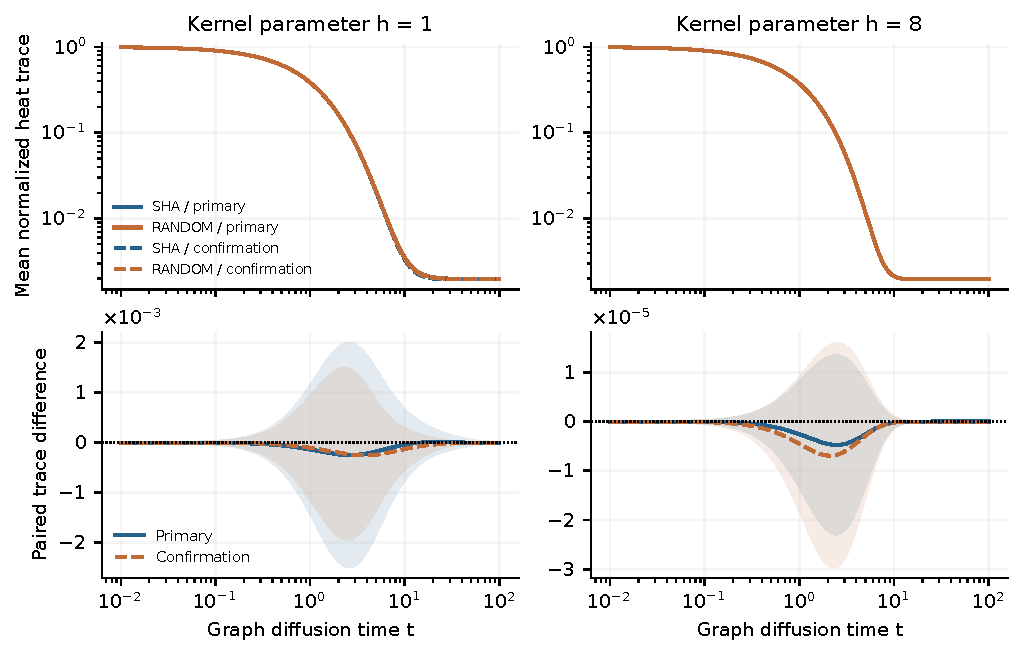
\includegraphics[width=\linewidth]{figures/heat_profiles.pdf}
\caption{Heat-kernel profiles from all 512 eigenvalues per graph. Top: mean normalized trace $Z(t)/512$ for SHA and random states in each group. Bottom: mean paired SHA-minus-random trace contrast; shading shows one standard deviation of dataset-level paired differences, not a confidence interval. The two kernel parameters yield different diffusion profiles. Close population means are descriptive comparisons, not a test of equivalence.}\label{fig:heat}\end{figure}

\subsection{What geometry means in this study}
Geometry here has an operational meaning: the metric, weighted neighborhoods and diffusion operator just defined, together with distances along intervention trajectories. These are concrete structures that can be measured without first identifying a smooth manifold. Continuum heat-kernel analysis~\cite{grigoryan} provides mathematical background; transferring an intrinsic-curvature or topology interpretation to these data requires a separate correspondence between that object and the measured graph.

The finite-graph diagonal is nonincreasing because its derivative is $-\sum_j\lambda_j e^{-t\lambda_j}\phi_j(i)^2\leq0$. A two-time diagonal ratio therefore does not establish the sign of an underlying manifold's scalar curvature. Likewise, a Poincar\'e representation with prescribed negative curvature imposes a metric. When binary sign vectors are projected to a common radius, the resulting distance is a monotone function of Hamming distance. Neither construction alone demonstrates an intrinsic hyperbolic manifold.

\FloatBarrier
\subsection{Replication and results}
Each primary replication uses a new seed and independently generated SHA inputs and random bits. We use percentile bootstrap intervals with 5,000 resamples of the paired dataset-level differences. These are descriptive, unadjusted intervals. They do not treat graph edges or eigenmodes as independent observations.

Table~\ref{tab:heat} evaluates the heat trace itself at the four saved diffusion times for each bandwidth and group. All sixteen paired intervals contain zero. This is a bounded negative result for the mean trace at the tested scales, not an equivalence test for spectra or kernels. The times were part of the original graph protocol; these interval summaries were added after inspection of the saved spectra.

\begin{table}[!htbp]\centering\small
\caption{SHA-minus-random mean heat trace, 20 dataset pairs per group. Multiply the estimate and both interval endpoints by the row's scale to obtain raw trace units; Figure~\ref{fig:heat} instead uses trace divided by 512. Intervals are descriptive 95\% paired bootstrap intervals.}\label{tab:heat}
\begin{tabular}{@{}lrrcrl@{}}\toprule
Group & $h$ & $t$ & Scale & Estimate & 95\% interval \\\midrule
\HeatTraceRows\bottomrule\end{tabular}\end{table}

\begin{figure}[!htbp]\centering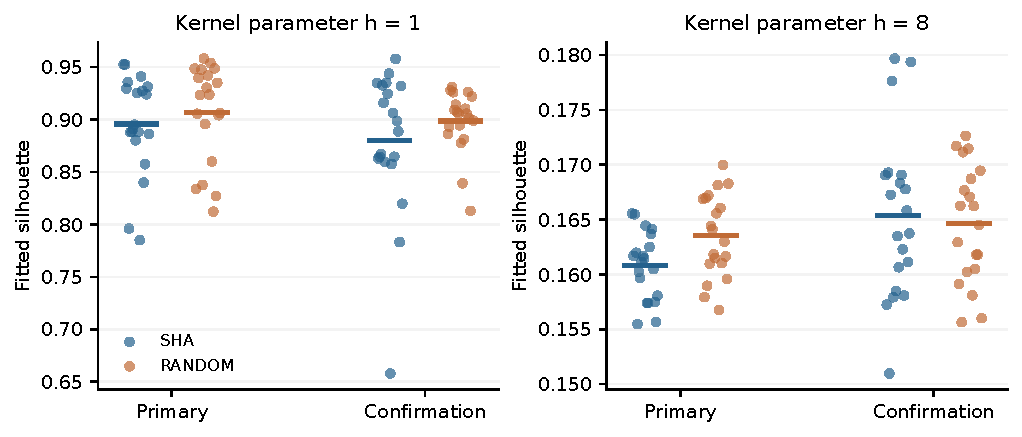
\includegraphics[width=\linewidth]{figures/graph_controls.pdf}
\caption{Each dot is one dataset's fitted silhouette; short bars show means. The same pipeline produces high scores in SHA and random data at $h=1$. Broadening the kernel changes the score substantially in both populations. The confirmation group uses fresh seeds.}\end{figure}

\begin{table}[!htbp]\centering\small
\footnotesize
\caption{Graph statistics, with SHA-minus-random differences and descriptive 95\% bootstrap intervals. Every row has 20 paired dataset replications.}
\begin{tabular}{@{}lllr r l@{}}\toprule
Group & $h$ & Statistic & SHA & Random & Difference [95\% interval] \\\midrule
\GraphRows
\bottomrule\end{tabular}\end{table}

The kernel parameter changes mean silhouette from approximately 0.90 to 0.16 in both populations. At $h=1$, the primary mean sorted cluster sizes are $(2.00,2.05,2.30,3.65,502.00)$ for SHA and $(2.00,2.05,2.10,3.55,502.30)$ for random data. The confirmation group has the same extreme imbalance, with mean largest clusters 500.95 and 501.85. The score therefore describes a dominant cluster and a few very small groups in the fitted coordinates; it is not evidence for five substantive state populations or for a disconnected graph. At $h=8$, primary mean sorted sizes range from 86.4 to 121.2 for SHA and 81.35 to 121.05 for random data. The primary $h=8$ silhouette difference is slightly negative; that contrast does not repeat in the confirmation group. The spectral-gap intervals include zero in both groups at both kernel parameters.

The detour contrast is more nuanced. Its small negative interval repeats in the first two groups. We therefore retain that observation rather than replacing it with a claim of equality. A further twenty-dataset sensitivity sample compares working states and actual digests with both PCG64 and MT19937 references (Table~\ref{tab:sensitivity}). Those intervals include zero, and the estimates vary with representation and reference. These observations already weaken the contrast, and the 100-pair follow-up reported below does not reproduce it; none of these samples establishes a robust general fingerprint.

\begin{table}[!htbp]\centering\small
\caption{Fresh detour sensitivity sample, 20 paired replications per comparison. State means terminal pre-feed-forward working state. These follow-up comparisons were specified after observing the first two graph groups.}\label{tab:sensitivity}
\begin{tabular}{@{}lrr@{}}\toprule
Comparison & Mean difference & 95\% interval \\\midrule
\SensitivityRows\bottomrule
\end{tabular}\end{table}

The confirmation and sensitivity samples are follow-ups, not a preregistered external replication. Their protocols and seeds were saved before their execution. Reporting each group separately preserves the distinction between initial exploration and fresh evaluation without assuming that a later nonsignificant interval disproves an earlier effect.

A further author-run sample uses 100 fresh seeds, 263910--264009, with the same four representations and graph construction (Table~\ref{tab:freshdetour}). Its working-state-minus-PCG64 estimate is \FreshDetourMean{}, with interval \FreshDetourCI{}; all five intervals contain zero. The earlier negative contrast was not reproduced in these 100 pairs. We retain the earlier estimates and do not interpret this outcome as proof of identical populations. This follow-up was specified after external review; its seeds are separate from the reviewer's own run, which is not included in these results.

\begin{table}[!htbp]\centering\small
\caption{Additional detour follow-up: 100 new dataset pairs, 512 points per dataset. All differences use the original detour definition and descriptive 95\% paired bootstrap intervals.}\label{tab:freshdetour}
\begin{tabular}{@{}lrr@{}}\toprule Comparison & Mean difference & 95\% interval \\\midrule
\FreshDetourRows\bottomrule\end{tabular}\end{table}

\section{Coordinate-resolved avalanche and selection}
The spectral experiment describes relations among terminal states. We next follow local changes through the computation itself. Neighboring input messages start one bit apart; their state separation becomes a trajectory indexed by compression round and input coordinate. This is the dynamical side of the geometric investigation. It concerns aggregate Hamming response, distinct from requiring each output bit to satisfy the strict avalanche criterion~\cite{webster}.
For each base message $m$ and input bit $i$, we measure
\begin{equation}A_r(m,i)=\operatorname{HW}\bigl(X_r(m)\oplus X_r(m\oplus e_i)\bigr),\end{equation}
where $\operatorname{HW}$ counts changed bits across all eight working words. This is a physical input intervention with a declared output statistic. It is not a per-output-bit diffusion rate.

Every one of 128 discovery bases is perturbed at all 440 content positions. The 22 positions with smallest discovery mean $A_{24}$ are frozen before evaluating a separate set of 128 bases. Selecting 22 positions defines a candidate set; the count is not itself a test for exceptional bits. Resampling is over bases, keeping all within-base interventions together.

\begin{figure}[!htbp]\centering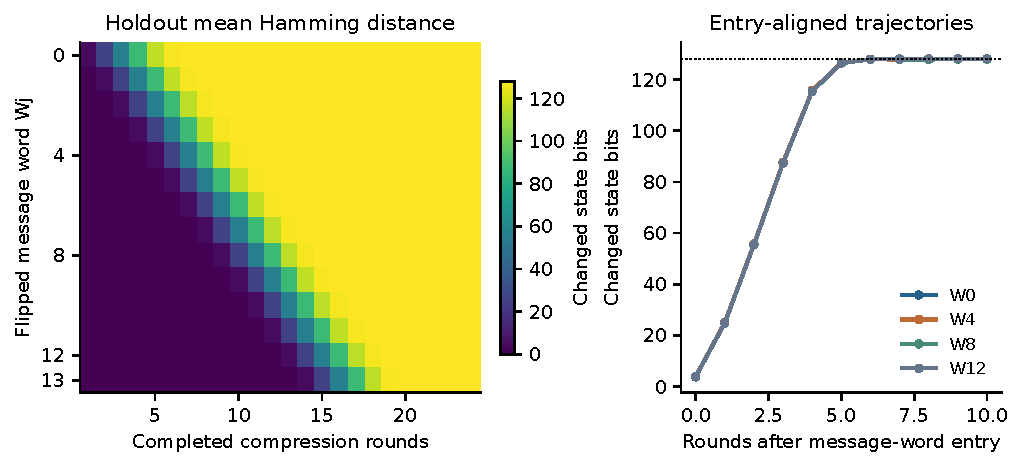
\includegraphics[width=\linewidth]{figures/avalanche_entry.pdf}
\caption{Measured holdout avalanche. Left: mean Hamming distance grouped by the actual flipped message word. Right: selected word groups aligned by their entry round. Later words begin influencing the state later; a full-trajectory slope would combine that delay with growth and saturation.}\end{figure}

The entry-aligned view exposes a common progression across the displayed word groups: an initially localized change spreads through the state and approaches a separation near 128 bits. This is a measured organization of the response in time and input coordinates. It also changes the question we should ask of a purportedly slow direction. A coordinate that enters later has had less time to act; a coordinate with a small sample mean must still be evaluated on new bases. The trajectory supplies the structure, and the holdout asks whether a selected feature travels beyond the sample that suggested it.

The selected-minus-other holdout difference at round 24 is \HoldoutDifference{} bits, with interval \HoldoutCI{}. The discovery--holdout correlation across the 440 position means is \RoundCorrelation{}. Their holdout standard deviation is \PositionSD{} bits, compared with an estimated sampling contribution of \NoiseFloor{} bits. To account for shared bases, this estimate uses $[\sum_i\widehat{\operatorname{Var}}_b(A_{24}(b,i)-\bar A_{24}(b,\cdot))/(128\times439)]^{1/2}$, with sample variances over bases. These observations are consistent with sampling-scale variation and establish no persistent lower-distance advantage at this resolution. They do not make a null result inevitable. Across the holdout interventions, mean round-64 Hamming distance is \FinalHamming{} bits out of 256.

\subsection{Early-round structure within one message word}\label{sec:early}
Within W0, every coordinate enters at the same round. The early response nonetheless depends reproducibly on the position within that word (Table~\ref{tab:earlycoord}). Across rounds 1--5, the correlation of discovery and holdout position means is 0.930--0.979, and offset 0 is the smallest in both partitions. The correlation is still 0.557 at round 6 and is near zero at round 7; these samples do not define a universal disappearance threshold. This analysis was chosen after inspecting the frozen arrays and uses their existing independent partitions, not a third validation sample.

\begin{table}[!htbp]\centering\small
\caption{Original one-bit interventions restricted to W0; 128 bases in each partition. Correlation is across 32 position means. MSB and W0 mean are holdout Hamming counts; minimum columns report MSB-first offsets.}\label{tab:earlycoord}
\begin{tabular}{@{}rrrrrr@{}}\toprule
Round & Correlation & MSB mean & W0 mean & Discovery min & Holdout min \\\midrule
\EarlyCoordinateRows\bottomrule\end{tabular}\end{table}

The round-1 endpoint has an exact explanation. Flipping the MSB of $W_0$ changes it by $2^{31}$ modulo $2^{32}$. At the first step, $T_1$ contains $W_0$ additively and the other inputs are unchanged, so both $a_1=T_1+T_2$ and $e_1=d_0+T_1$ change by $2^{31}$. Adding that value toggles precisely the MSB of a 32-bit word. The other six working words are unchanged, giving $A_1(m,0)=2$ for every base. Both saved partitions satisfy this identity. Lower-position additions can also affect more significant bits through carries. This explains the exceptional first-step MSB response; later rounds combine carries, rotations and Boolean mixing, and the data alone do not assign every later effect to one mechanism.

\subsection{Candidate provenance and equal-budget search}

We separately test the fixed candidate positions $S=\{1,5,7,9,10,14\}$ on 256 fresh bases. This set is carried over from the author's exploratory analyses and is fixed before the present evaluations; it is not selected from the graph spectra or tuned on these holdouts. Its members occupy the more significant part of W0, so significance must be considered when interpreting a response difference. For each six-position set, the search evaluates all 15 two-position flips and retains the smallest raw round-24 Hamming distance. The comparator comprises twenty uniformly sampled six-position subsets of W0, with exactly the same search budget. Distances are left on the same scale on both sides.

\begin{figure}[!htbp]\centering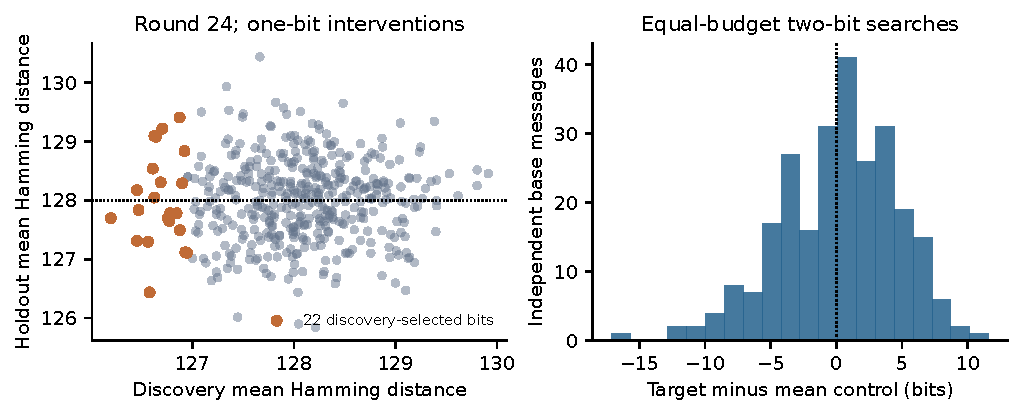
\includegraphics[width=\linewidth]{figures/holdout_search.pdf}
\caption{Independent evaluation of selected coordinates. Left: discovery versus holdout means for all 440 positions, with the frozen 22 highlighted. Right: per-base candidate-minus-control difference for equally budgeted two-bit searches; negative values favor the candidate.}\end{figure}

The candidate-minus-mean-control difference is \SearchDifference{} bits, with interval \SearchCI{}. This comparison does not resolve an advantage for the tested candidate. The interval is conditional on the twenty sampled control sets; it does not quantify uncertainty over every possible six-position set. The search question remains distinct from digest discrimination or attack complexity.

The fresh early-round follow-up fixes rounds 2--7 and 24 before execution, draws 256 new bases and twenty new uniform W0 control sets, and saves all fifteen pattern scores per set, base and round. Against these uniform controls, Table~\ref{tab:earlysearch} shows smaller candidate minima at rounds 2--5, with intervals below zero; rounds 6, 7 and 24 do not resolve a difference. Matching entry time and search budget does not match bit significance, and Section~\ref{sec:early} shows that early response depends on position within the word. The candidate occupies offsets 1--14, the more significant half of W0, whereas uniform controls mix both halves; at round 2 the uniform-control means correlate \UniformSearchOffsetCorr{} with the mean offset of the control set. A second control family therefore draws forty six-position subsets of offsets 0--14 with a saved seed and evaluates them on the same bases. Against these significance-matched controls the sign reverses: the candidate minimum is larger by \MatchedSearchDiffTwo{} bits at round 2, with interval \MatchedSearchCITwo{}, and \MatchedSearchBelowTwo{} of the forty matched sets have smaller minima than the candidate. Rounds 3 and 4 behave the same way; against the matched family, rounds 5--7 and 24 do not resolve a difference. The early distance reduction is thus a property of significant positions, not of this candidate, and it is not evidence of a distinct $\Sigma_0$ mechanism or of reduced collision or preimage complexity. All intervals are descriptive, unadjusted and conditional on the sampled sets.

\begin{figure}[!htbp]\centering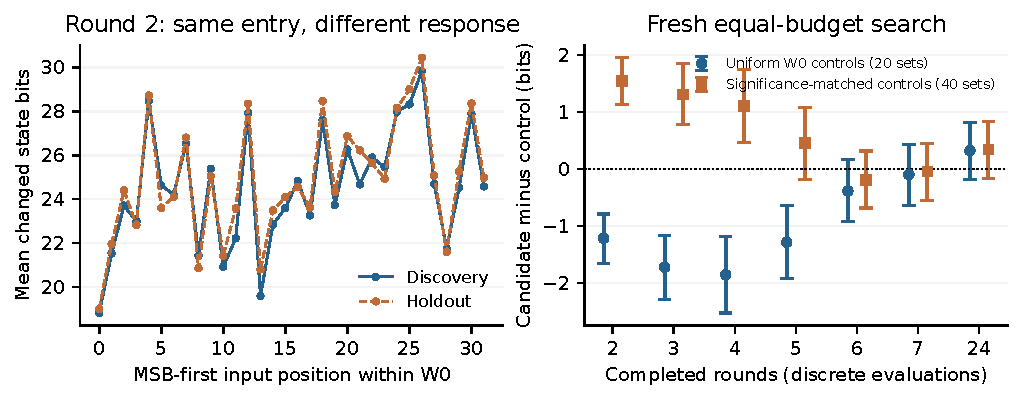
\includegraphics[width=\linewidth]{figures/early_structure.pdf}
\caption{Early structure and its independent evaluation. Left: round-2 one-bit response within W0 in the two original partitions. Right: fresh equal-budget search differences against the twenty uniform W0 control sets and the forty significance-matched sets, with descriptive 95\% base-bootstrap intervals; negative favors the candidate. Round positions on the right are discrete evaluations, not a continuous time axis.}\end{figure}

\begin{table}[H]\centering\small
\caption{Fresh two-bit searches, 256 bases. Each set receives fifteen patterns per base; counts are minimum Hamming distance across eight working words. Uniform: twenty six-position subsets of all of W0. Matched: forty six-position subsets of offsets 0--14, evaluated on the same bases. Differences are candidate minus control mean; negative favors the candidate. The last column counts matched sets whose mean minimum is below the candidate's.}\label{tab:earlysearch}
\begin{tabular}{@{}rrrlrlr@{}}\toprule Round & Cand. & Uniform & Diff. [95\%] & Matched & Diff. [95\%] & Sets below \\\midrule
\EarlySearchRows\bottomrule\end{tabular}\end{table}

\section{Cube measurements and the timing of interventions}
For a declared set of $k$ input coordinates $S$, the cube sum of an output $f$ is its $k$-fold Boolean derivative,
\begin{equation}\Delta_S f(m)=\bigoplus_{u\in\{0,1\}^{k}}f(m\oplus E_Su).\end{equation}
A Boolean polynomial of total degree below $k$ has zero $k$-fold derivative~\cite{lai}. A zero sum on a particular cube does not, conversely, prove a global degree bound. Cube attacks~\cite{dinur} and cube testers~\cite{testers} use related algebraic tools with different objectives. Our zero-rate measurements are cube tests on working-state projections; they do not perform key extraction or construct collisions or preimages.

\subsection{Candidate cubes with matched entry time}
We compare the candidate set $S$ with twenty random six-position subsets of W0. All variables therefore enter at the same compression step. The same 512 independently generated 55-byte bases are used for every set. Each cube evaluates 64 corners. The observable is the XOR sum of bit 16, numbered from the least-significant end, of register $a$. A zero bit-sum has reference probability one half under the random-function comparison.

\begin{table}[!htbp]\centering\small
\caption{Six-bit cube results. Differences and intervals are percentage points. The last column adjusts the eight candidate-versus-one-half binomial tests by Holm's method; it is not a test of the candidate-versus-control difference.}
\begin{tabular}{@{}rrrrlr@{}}\toprule
Round & Candidate (\%) & Control (\%) & Difference & 95\% interval & Holm $p$ \\\midrule
\CubeRows\bottomrule
\end{tabular}\end{table}

None of the eight candidate zero-rate tests rejects after the stated adjustment. Every paired candidate-minus-control interval also includes zero. This supports a bounded negative result for this set, projection, background distribution and sample size. It does not show equivalence to all controls or bound the best cube over all coordinates and observables.

\FloatBarrier
\subsection{Fresh early-round cube tests}
To examine the period before aggregate avalanche saturation, the follow-up fixes rounds 2--7 in addition to the original eight round counts. It draws 512 new bases and twenty new six-position W0 control sets. The candidate and output projection remain fixed, and the code saves all eight word sums as well as the single-bit indicators. The fourteen candidate-versus-one-half tests form a separate Holm-adjusted family. Paired candidate-minus-control intervals remain descriptive and conditional on the sampled sets.

At round 2, the candidate zero rate is \EarlyCubeTarget\%, versus \EarlyCubeControl\% averaged over the twenty uniform controls; the paired difference is \EarlyCubeDifference{} percentage points, with interval \EarlyCubeCI{}. The remaining thirteen uniform-control intervals contain zero (Table~\ref{tab:earlycube}). Three observations bound the interpretation. First, the uniform-control mean is itself far above one half at round 2, and the twenty uniform sets range from \UniformCubeMinTwo\% to \UniformCubeMaxTwo\%; a candidate-versus-one-half test at this round measures the round, not the candidate, so its adjusted $p$-value of \EarlyCubeP{} is not evidence of a candidate-specific effect. Second, every candidate position is more significant than the observed bit 16, and the round-2 zero rate of a uniform set increases with the number of its positions above bit 16 (correlation \UniformCubeAboveCorr{}). Against the forty significance-matched sets, evaluated on the same bases, the candidate rate lies inside the control range \MatchedCubeRangeTwo\%, with \MatchedCubeAtOrAboveTwo{} matched sets at or above it; the paired difference against the matched mean of \MatchedCubeMeanTwo\% is \MatchedCubeDiffTwo{} points, with interval \MatchedCubeCITwo{}, which places the candidate near the middle of its class rather than outside it. Third, the zero rate is a single-bit property: the complete word sum of register $a$ is zero for \WholeWordATwo\% of bases with the candidate and \WholeWordAControlTwo\% with uniform controls. Rounds 3--24 do not resolve a candidate-minus-control difference against either family; one matched interval, at round 7, marginally excludes zero among fourteen unadjusted comparisons, and the candidate-versus-one-half test at that round does not reject after adjustment. Neither the control means nor the candidate rate proves a global algebraic-degree bound.

\begin{table}[!htbp]\centering\small
\caption{Fresh six-bit cube tests, 512 bases; zero rate of the six-fold derivative of bit 16 of register $a$, in percent. Uniform: twenty subsets of all of W0. Matched: forty subsets of offsets 0--14 on the same bases. Differences and intervals are percentage points. The sets column counts matched sets with zero rate at or above the candidate's. Holm $p$ adjusts the fourteen candidate-versus-one-half tests; at round 2 it reflects the round, not the candidate.}\label{tab:earlycube}
\footnotesize\begin{tabular}{@{}rrrlrlrr@{}}\toprule
Round & Cand. & Uniform & Diff. [95\%] & Matched & Diff. [95\%] & Sets $\geq$ cand. & Holm $p$ \\\midrule
\EarlyCubeRows\bottomrule\end{tabular}\end{table}

These tests identify a round-2 bias in the single-bit six-fold derivative for almost every tested six-position set, strongest for sets drawn from the more significant half of W0, with the candidate an ordinary member of that family. The single-bit six-fold derivative has its own behavior: the whole-word three-bit entry control below cannot determine whether this different observable is balanced. Nor does a mean one-bit Hamming distance near 128 imply randomness of every higher-order response. The later-round rows remain measurements of those observables rather than consequences assumed from saturation.

\FloatBarrier
\subsection{Coupled register families and perturbation transport}
An input variable in original message word $W_j$ first enters at compression step $j$, or completed-round count $j+1$. We use $\delta=r-(j+1)$ to describe time since that entry. A separate control draws 256 uniform raw 64-byte blocks and moves the same three MSB-first offsets $\{0,1,2\}$ among W0, W4, W8, W12 and W15. These are raw compression-block interventions, including positions that would be padding or length bits in a message-based experiment; no padded-message interpretation is applied.

The working state has a useful algebraic organization into $A_r=(a_r,b_r,c_r,d_r)$ and $E_r=(e_r,f_r,g_r,h_r)$. Each family has a newly computed leading word and three transported words. With all additions taken modulo $2^{32}$, the two leading updates are~\cite{nist}
\begin{align}
 T_{1,r}&=h_{r-1}+\Sigma_1(e_{r-1})+\operatorname{Ch}(e_{r-1},f_{r-1},g_{r-1})+K_{r-1}+W_{r-1},\\
 T_{2,r}&=\Sigma_0(a_{r-1})+\operatorname{Maj}(a_{r-1},b_{r-1},c_{r-1}),\\
 a_r&=T_{1,r}+T_{2,r},\qquad e_r=d_{r-1}+T_{1,r}.
\end{align}
Here $\Sigma_0,\Sigma_1,\operatorname{Ch},\operatorname{Maj}$ and $K_j$ have their FIPS definitions, and $W_j$ is the expanded schedule word after the original sixteen input words. The shared $T_{1,r}$ and the $d_{r-1}$ term explicitly couple the families. This partition identifies two interacting parts of one state, not statistically independent systems.

The remaining updates copy working registers between rounds:
\begin{equation}
 b_r=a_{r-1},\quad c_r=a_{r-2},\quad d_r=a_{r-3},\qquad
 f_r=e_{r-1},\quad g_r=e_{r-2},\quad h_r=e_{r-3}.
\end{equation}
For the same base and intervention, cube differentiation commutes with these identities. Thus $\Delta_S d_r=\Delta_S a_{r-3}$ and $\Delta_S h_r=\Delta_S e_{r-3}$ whenever the displayed histories are defined. A trailing register can retain a zero sum after a leading register changes through exact transport. These identities give the observed pattern a precise meaning: the register view contains delayed copies of leading-word responses, while the nonlinear updates continually couple the two families.

\begin{figure}[!htbp]\centering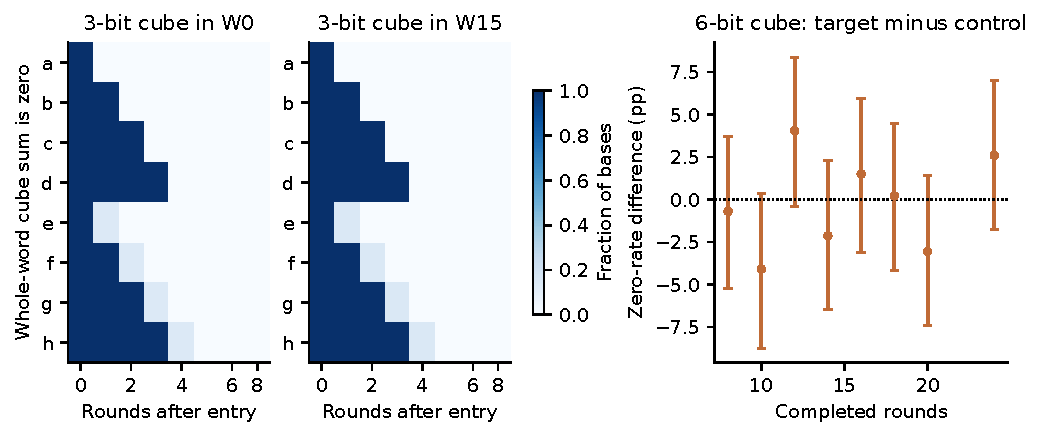
\includegraphics[width=\linewidth]{figures/cube_controls.pdf}
\caption{Two distinct cube observables. Left and center: fraction of raw bases with a whole-word zero sum for the three-bit entry control, aligned to variable entry; W0 and W15 illustrate the transport pattern. Right: single-output-bit zero-rate differences for the six-bit candidate experiment, with base-resampled 95\% intervals. A whole-word zero and a zero bit have different reference probabilities.}\end{figure}

The entry control displays the leading-to-trailing sequence predicted by the register identities. Its exact zero fractions depend on the selected offsets and backgrounds, so we do not identify a universal round threshold. Total round count alone is an incomplete description of the experiment: both the entry time of the variables and the observation register are necessary to interpret a surviving cube sum.

\section{Held-out classification of actual digests}
The classification experiment uses $H(m)$ rather than $X_{64}(m)$. Each of five independent replications contains 2,000 SHA digests and 2,000 independent random-bit strings for training, and another balanced 4,000-observation holdout. The fixed models are a 100-tree random forest with maximum depth ten and an RBF SVM with $C=1$, default scaled gamma and fifty PCA components. PCA is fitted on training observations only. No model or feature selection uses the holdout. Neural differential distinguishers, such as Gohr's work on reduced Speck~\cite{gohr}, use chosen-difference pair distributions and are a different experiment; our two classifiers are not a replication of that approach.

\begin{table}[!htbp]\centering\small
\caption{Five independent classifier replications. Ranges describe the five fits and are not confidence bounds on all distinguishers.}
\begin{tabular}{@{}lrrr@{}}\toprule
Model & Mean accuracy (\%) & Accuracy range (\%) & Mean AUC \\\midrule
\MLRows\bottomrule\end{tabular}\end{table}

\begin{figure}[!htbp]\centering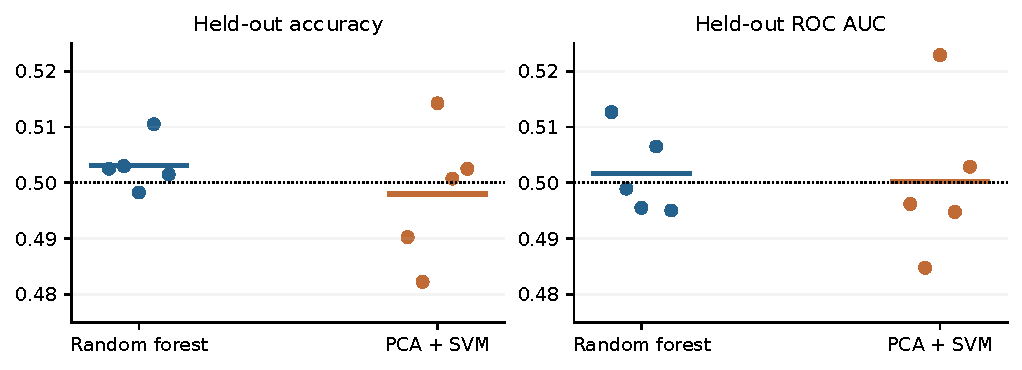
\includegraphics[width=\linewidth]{figures/digest_classifiers.pdf}
\caption{Each dot is a model trained and evaluated on a fresh balanced dataset. Horizontal colored bars indicate means; the dotted line is one-half. These results quantify the tested procedures, rather than cryptographic indistinguishability.}\end{figure}

The observed means are close to chance, with individual fits varying on either side. This experiment has finite sample size and limited model classes. It supplies no basis for inferring full-round security from classifier failure, nor does it invalidate a different statistic evaluated on a different object.

\section{Geometric interpretation and research direction}
Heat-kernel cryptanalysis begins by making the geometry of an observation explicit. In this study, that means a distance on bit states, a weighted neighborhood graph, and an operator whose modes resolve different diffusion scales. Following actual input perturbations adds a temporal description: entry, growth, transport and saturation. Taken together, these measurements let us describe where organization resides and ask which parts survive a change of sample or reference.

The dynamical measurements resolve reproducible early structure within a word even when input entry is held fixed. The exact MSB endpoint and the discovery--holdout coordinate agreement give that description an algebraic and an empirical anchor. The early equal-budget searches and round-2 cube tests add a boundary: a candidate drawn from the significant half of the word behaves like other sets of that class, so early advantage belongs to position, not to the candidate. The entry-aligned avalanche trajectories and cube-transport identities describe additional aspects of perturbation movement. They are complementary observables, not interchangeable definitions of diffusion. This combination provides a concrete starting point for investigating more detailed local geometry.

The terminal-state graph results have a different interpretation. Both SHA and random states acquire highly unbalanced fitted clusters at narrow bandwidth, and none of the sixteen tested mean heat-trace comparisons resolves a difference. The earlier detour contrast is not reproduced in the additional 100 pairs. The early position effects coexist with round-24 selection results that do not resolve a benefit and actual-digest classifier means near chance. This gives the investigation a temporal and observational scope; it supplies neither a full-round attack nor a security proof.

\subsection{From heat kernels to dual torus and double cover}\label{sec:continuity}
The connection that matters to my broader work is that one computation admits multiple connected descriptions. A state can be examined through its neighborhood relations, through a local intervention, or through the coupled register families that produce its next update. Each description preserves some information and suppresses other information. Understanding how they constrain one another became the next research question.

This line of investigation led me to the dual-torus formulation: to study the $A$ and $E$ families as coupled modular-coordinate systems and ask whether their local responses require different geometric descriptions. The modular arithmetic and the coupling equations above are the starting objects. Establishing a particular torus model, a carry-based geometry or distinct subsystem timescales requires the definitions and experiments of that subsequent work. The two-family partition by itself does not establish those further results.

The later double-cover work pursued the broader idea of different, connected descriptions belonging to the same object. Here that connection is motivation, not a topological conclusion: a double cover requires specified spaces and a map with the corresponding covering properties. Two register families or two ways of plotting a computation do not supply such a map. What this paper contributes to that progression is the initial investigative method and a concrete computational setting in which relationships between descriptions can be measured.

My purpose in this first study is to make the geometric question accessible to experiment. The next step is to ask whether a feature resolved in one description predicts a response in another, with the correspondence and the evaluation fixed in advance. Examples include relating a graph mode to a held-out intervention response, or testing a channel-specific observable after aligning input entry and register delay. These would connect the geometric and algebraic views more tightly than an absolute clustering score or a visually distinctive trajectory alone.

\subsection{Evidence and reproducibility}

The accompanying \texttt{sha256\_reproducibility.zip} supplies the exact main-run source snapshot, follow-up runners including the significance-matched control family, protocols, seeds, dependency versions, full graph spectra, intervention arrays, cube indicators, classifier holdouts and predictions, figure builder and manuscript source. Every numerical table and figure is generated from those records. All experimental inputs are synthetically generated; their generation code and seeds are included.

All bootstrap intervals use independently sampled bases or whole dataset pairs as the resampling unit. Most are descriptive and unadjusted; the original eight cube binomial tests and the fourteen follow-up tests each use Holm adjustment within their respective families. The shared candidate/control bases and sampled control sets are retained. The early-coordinate analysis reuses saved discovery and holdout arrays; fresh search, cube and detour protocols were saved before execution but chosen after earlier results and review; the significance-matched control family was added after a second review, with its protocol, seed and set count saved before execution. All follow-up rounds are reported. These design boundaries delimit the findings without converting the paper into a claim about every possible SHA-256 measurement.

\paragraph{Funding.} This research received no external funding.

\begin{thebibliography}{99}
\bibitem{nist} National Institute of Standards and Technology. \emph{Secure Hash Standard (SHS)}. FIPS PUB 180-4, 2015. \url{https://doi.org/10.6028/NIST.FIPS.180-4}.
\bibitem{luxburg} U. von Luxburg. A tutorial on spectral clustering. \emph{Statistics and Computing}, 17:395--416, 2007. \url{https://arxiv.org/abs/0711.0189}.
\bibitem{dinur} I. Dinur and A. Shamir. Cube attacks on tweakable black box polynomials. \emph{EUROCRYPT 2009}, pp. 278--299. Preprint: \url{https://eprint.iacr.org/2008/385}.
\bibitem{belkin} M. Belkin and P. Niyogi. Laplacian eigenmaps for dimensionality reduction and data representation. \emph{Neural Computation}, 15(6):1373--1396, 2003. \url{https://doi.org/10.1162/089976603321780317}.
\bibitem{coifman} R. R. Coifman and S. Lafon. Diffusion maps. \emph{Applied and Computational Harmonic Analysis}, 21(1):5--30, 2006. \url{https://doi.org/10.1016/j.acha.2006.04.006}.
\bibitem{sun} J. Sun, M. Ovsjanikov and L. Guibas. A concise and provably informative multi-scale signature based on heat diffusion. \emph{Computer Graphics Forum}, 28(5):1383--1392, 2009. \url{https://doi.org/10.1111/j.1467-8659.2009.01515.x}.
\bibitem{grigoryan} A. Grigor'yan. \emph{Heat Kernel and Analysis on Manifolds}. AMS/IP Studies in Advanced Mathematics, vol. 47, 2009. \url{https://doi.org/10.1090/amsip/047}.
\bibitem{webster} A. F. Webster and S. E. Tavares. On the design of S-boxes. \emph{CRYPTO '85 Proceedings}, LNCS 218, pp. 523--534, 1986. \url{https://doi.org/10.1007/3-540-39799-X_41}.
\bibitem{lai} X. Lai. Higher order derivatives and differential cryptanalysis. \emph{Communications and Cryptography}, pp. 227--233, 1994. \url{https://doi.org/10.1007/978-1-4615-2694-0_23}.
\bibitem{testers} J.-P. Aumasson, I. Dinur, W. Meier and A. Shamir. Cube testers and key recovery attacks on reduced-round MD6 and Trivium. \emph{FSE 2009}, LNCS 5665, pp. 1--22. \url{https://doi.org/10.1007/978-3-642-03317-9_1}.
\bibitem{lamberger} M. Lamberger and F. Mendel. Higher-order differential attack on reduced SHA-256. \emph{Cryptology ePrint Archive}, Report 2011/037. \url{https://eprint.iacr.org/2011/037}.
\bibitem{gohr} A. Gohr. Improving attacks on round-reduced Speck32/64 using deep learning. \emph{CRYPTO 2019}, pp. 150--179. \url{https://doi.org/10.1007/978-3-030-26951-7_6}.
\bibitem{mendel2013} F. Mendel, T. Nad and M. Schl\"affer. Improving local collisions: new attacks on reduced SHA-256. \emph{EUROCRYPT 2013}, LNCS 7881, pp. 262--278. \url{https://doi.org/10.1007/978-3-642-38348-9_16}.
\bibitem{li2024} Y. Li, F. Liu and G. Wang. New records in collision attacks on SHA-2. \emph{EUROCRYPT 2024}. Preprint: \url{https://eprint.iacr.org/2024/349}.
\bibitem{zhang2026} Z. Zhang, M. Li, L. Gao and M. Wang. Collision attacks on SHA-256 up to 37 steps with improved trail search. \emph{EUROCRYPT 2026}. Preprint: \url{https://eprint.iacr.org/2026/232}.
\bibitem{khovratovich2012} D. Khovratovich, C. Rechberger and A. Savelieva. Bicliques for preimages: attacks on Skein-512 and the SHA-2 family. \emph{FSE 2012}, LNCS 7549, pp. 244--263. \url{https://doi.org/10.1007/978-3-642-34047-5_15}.
\end{thebibliography}
\end{document}
